\chapter{Introduction}

\begin{goals}
\item Consider careers in computer science
\item Understand the basic history of computer science
\item Know the components of a computer
\item Understand the different types of computers
\end{goals}

Welcome to CS 103! In this course, you'll come to understand what makes computers tick. What are the different components inside a computer? How do they work together? How do different computers talk to each other? We'll answer all these questions and more, giving you a strong foundation for further study of information technology (IT) or computer science (CS). 

In addition, we'll spend lots of time learning how to control computers through \emph{programming}. The computer industry is continually growing, and companies need more and more programmers who are adept at instructing computers to manage information and carry out tasks. By the end of this course, you'll know how to write your own programs, and you'll be ready to keep studying programming and improve your skills.

In this chapter, we'll start with a broad overview of computers: what they are used for, their history, the parts that make them up, and the different types of computers.

\section{Why computers are useful}

Computers help us in most tasks in the modern age to make our lives easier and more comfortable. They are able to complete these tasks quickly and simultaneously. We can use them, for example, to:

\begin{itemize}
	\item Write a letter
	\item File taxes
	\item Play video games
	\item Browse the Internet
	\item Talk with friends
	\item Date
	\item Order food
	\item Control robots and self-driving cars
\end{itemize}

Computers are at the core of many endeavors to make meaningful differences in the world, whether through space exploration, medical advances, expanding communication, or furthering education. As computers become more embedded into our daily lives, it is increasingly important for everyone to understand how computers work, and how to use them. The job market for computer scientists and software engineers is continuing to expand, and computer skills are becoming more necessary even in non-computational jobs.

According to a 2018 survey\endnote{https://insights.stackoverflow.com/survey/2018/} on Stack Overflow, a very popular online community for software developers, 9\% of professional coders have only been coding for 0--2 years. This shows that it doesn't take too much time to become a coder, and that the job market for coders is continually expanding. Some examples of careers in computer science include:

\begin{itemize}
\item Information Technology (IT) manager/consultant: analyzes the technology needs of organizations and makes computer systems recommendations. (Base Salary: \$85,000 -- \$90,000)
\item Game developer: programs and develops console, computer, and mobile video games from concept to actual product. (Base Salary: \$52,000 -- \$127,000)
\item Web developer: takes a web design and turns it into a website by writing code in a variety of programming languages. (Base Salary: \$52,000 -- \$110,000)
\item UI/UX designer: UI stands for ``user interface'' and UX stands for ``user experience.'' UI designers focus on the look and layout of a product. UX designers focus on how a product works and how people interact with it. (Base Salary: \$59,000 -- \$110,000)
\item Data analyst: retrieves and organizes data to reach meaningful conclusions with statistical, coding, and analytical tools. (Base Salary: \$45,000 -- \$95,000)
\item Database manager: oversees an organization's data storage and retrieval system. (Base Salary: \$39,000 -- \$87,000)
\end{itemize}
In this course, you will learn how to program a computer -- that is, how to instruct the computer to perform tasks. The concepts and skills you learn in this course will form an important foundation that will make you a more informed citizen, and perhaps, a computing professional. 

\section{Brief history of computer science}

The history of inventions is complicated, with many twists and turns as scientists and engineers refined the concept of what a ``computer'' is and made technological advancements which aided in their construction. Assigning faces and dates to specific technologies that are often many years and people in the making is difficult. 
%For an excellent layman's survey of the history of computer science, check out ``The Innovators" by Walter Isaacson. 
Nevertheless, here is a brief summary of the major steps, which should give a general idea of when and where different innovations were made\endnote{https://www.livescience.com/20718-computer-history.html}:

\begin{itemize}
\item As early as the 1830's, Charles Babbage had the concept of a machine which could carry out computations automatically. He designed and built a machine called the Difference Engine, which could calculate the values of polynomial functions. Next he conceived of a more ambitious machine, the Analytical Engine shown to the right, which was designed for general-purpose computation. Unfortunately he did not complete its construction before his death.
\begin{marginfigure}
	\centering
	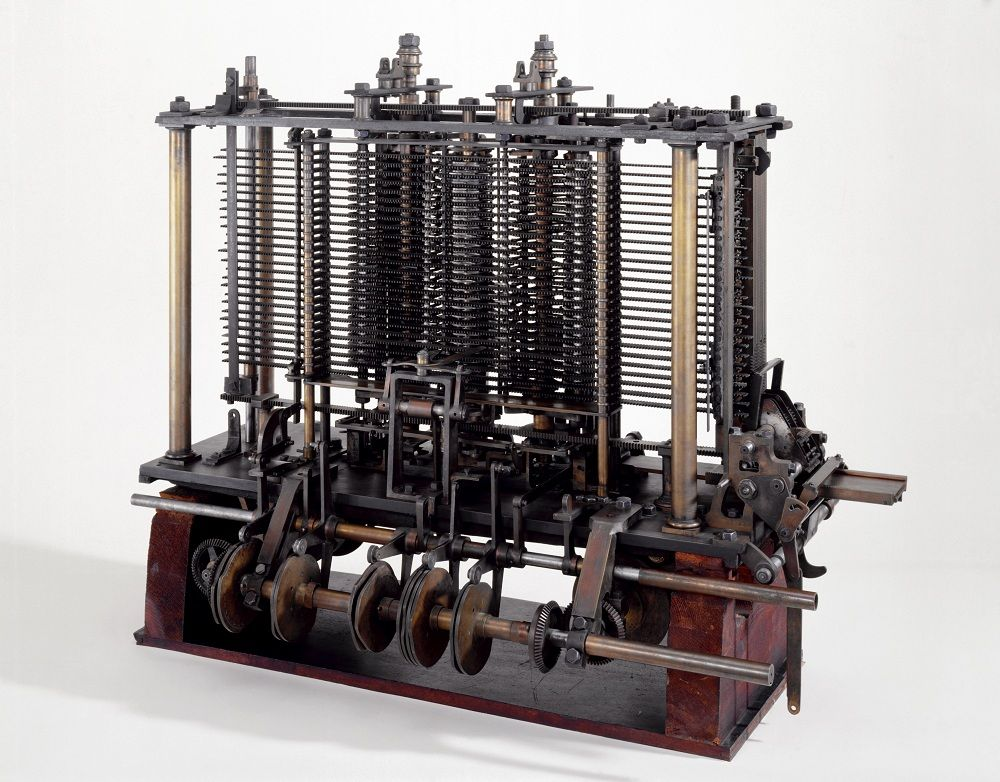
\includegraphics[width=\textwidth]{images/analytic_engine.jpg}
	\caption{Charles Babbage's Victorian-era computer, called the ``Analytical Engine.'' Ada Lovelace worked closely with Babbage and was inspired to imagine how powerful future computers would be.}
	\label{fig:analytic_engine}
\end{marginfigure}
Ada Lovelace, daughter of the poet Lord Byron, learned of the plans for the Analytical Engine. She recognized its many potential uses, and wrote a program which would have taught the machine how to carry out an advanced mathematical calculation. For this reason, Ada Lovelace is considered by many to be the first computer programmer.
\item About a century later in the 1930's, a British mathematician named Alan Turing explored the abstract idea of universal computation: a machine which could be programmed to simulate any other computing machine. Turing's idea is the theoretical basis for modern computers. When World War II began, Turing was called upon to build a version of his machine which could break the codes being used by Germany and the Axis Powers. 
\begin{marginfigure}
	\centering
	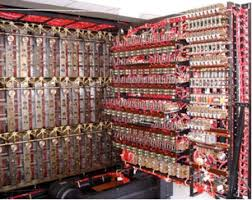
\includegraphics[width=\textwidth]{images/bombe.jpg}
	\caption{Alan Turing's code-breaking computer}
	\label{fig:bombe}
\end{marginfigure}
After the war, Turing returned to theoretical ideas, and began to wonder if computers could ever be made to ``think.'' Turing was one of the founders of the field known as artificial intelligence, which is expanding rapidly today.
\item During World War II, scientists and engineers in the United States built upon Turing's ideas, and improved the technology by building the first fully electronic general-purpose computer, called ENIAC. ENIAC was used by the United States Army to design and improve weapons, including nuclear weapons.
\begin{marginfigure}
	\centering
	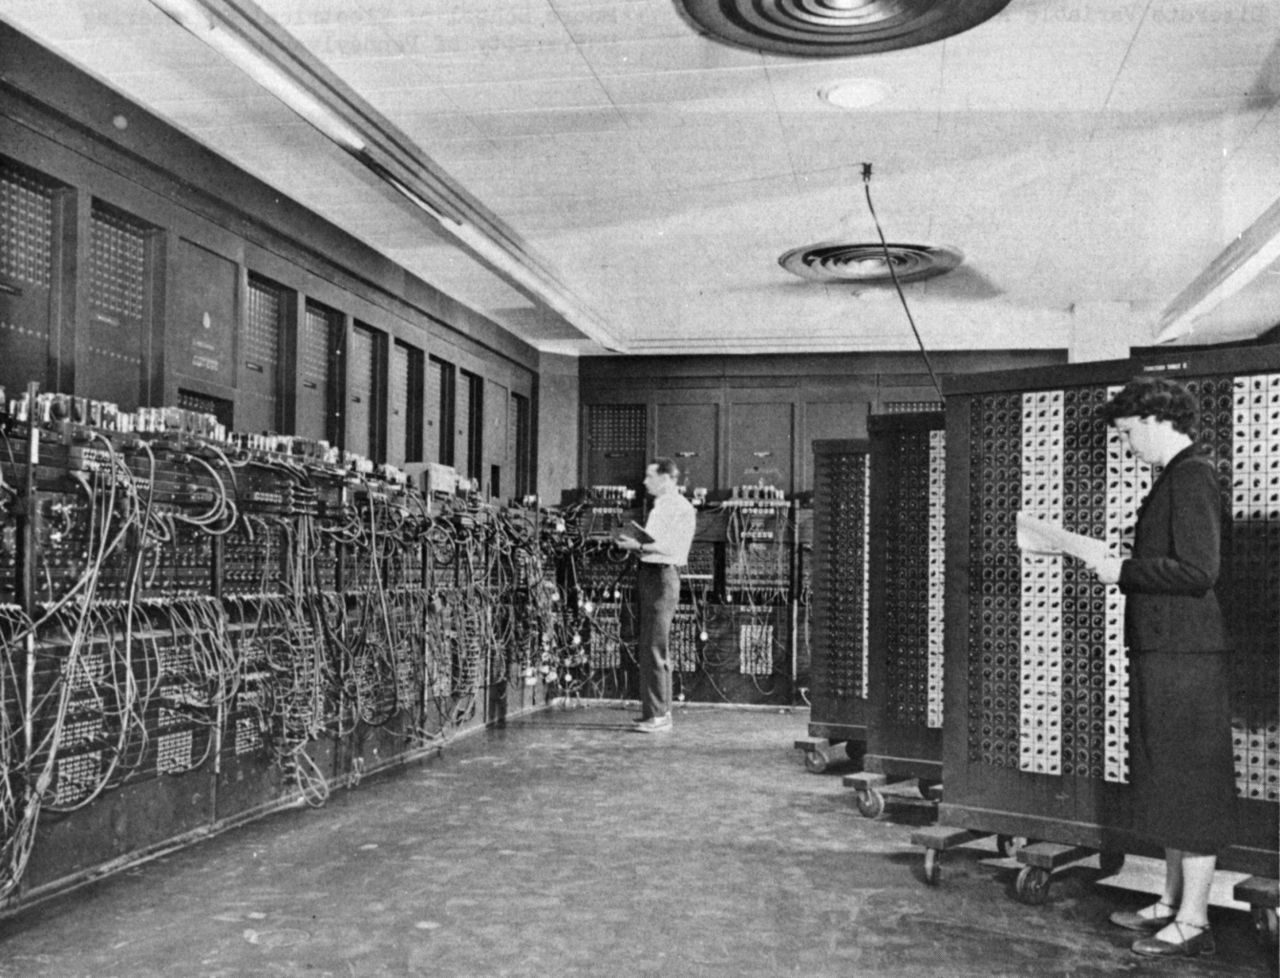
\includegraphics[width=\textwidth]{images/eniac.jpg}
	\caption{ENIAC, the first fully electronic computer, hosted at the University of Pennsylvania.}
	\label{fig:eniac}
\end{marginfigure}
\item In 1947, John Bardeen, Walter Brattain, and William Shockley succeeded in developing the first transistor, an electronic device which could replace the bulky vacuum tubes that had been used in ENIAC. This discovery won them the Nobel Prize in Physics, and allowed engineers to eventually shrink computers down to the size of a laptop or cell phone.
\item As computers became smaller and more affordable, more of them went into use, and it became important to have a way for computers to send data to each other. The United States Department of Defense designed and established the first major computer network, ARPANET, which connected several universities and laboratories across the country. The technology used in ARPANET forms the foundation for the modern Internet.
\item In 1975, Bill Gates and Paul Allen wrote software for a new kind of microcomputer which allowed them to run programs in a language called BASIC. They named their microcomputer software company Microsoft, and it became a major force in the growth of computers for personal use.
\item Shortly after, in 1977, Steve Wozniak and Steve Jobs pioneered the design of a computer engineered for usability by non-professionals. Their device, called the Apple II, was Apple's first computer intended for use in households rather than businesses.
\begin{marginfigure}
	\centering
	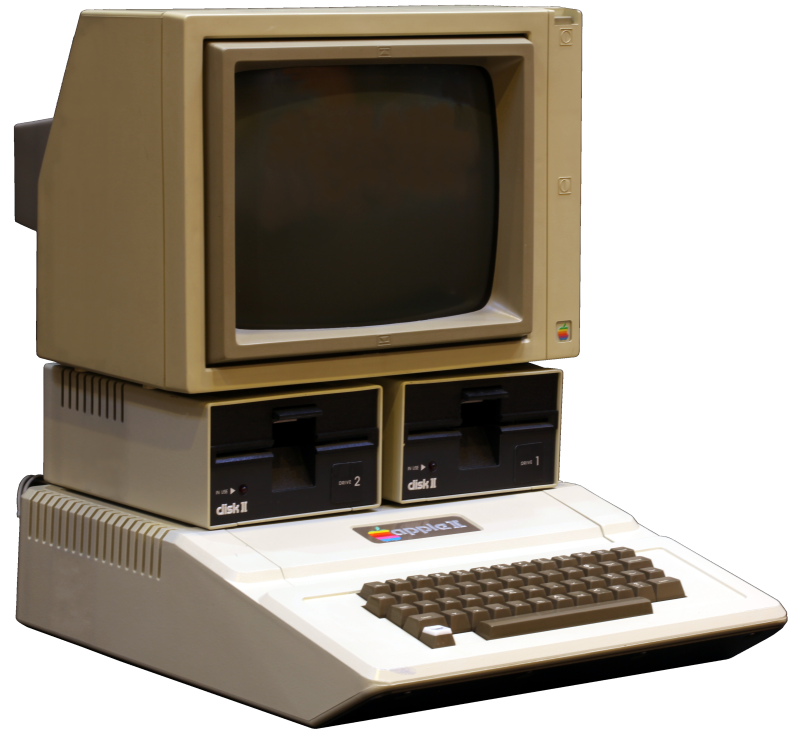
\includegraphics[width=\textwidth]{images/appleii.png}
	\caption{The Apple II, a computer built for use by non-professionals, and a precursor of modern personal computers.}
	\label{fig:appleii}
\end{marginfigure}
\item As personal computing expanded rapidly, private government and research networks like ARPANET no longer satisfied the demand for connecting computers. In 1990, Sir Tim Berners-Lee invented the World Wide Web, which allowed people to use their computers to view web pages hosted on other computers. The World Wide Web remains in use today, and has been a major driver in the growth of the computer industry.
\end{itemize}

\section{Components of a computer}

There are four primary components of a computer: its hardware, its software, its data, and its user. We'll cover each of these in more detail in later chapters, but we will give a brief overview here.

\subsection{Hardware}

Computer hardware consists of physical, electronic devices. These are the parts you actually can see and touch. Some examples (you don't need to memorize this list!) include\endnote{https://www.tutorialandexample.com/computer-hardware/}

\begin{itemize}
	\item Central processing unit (CPU)
	\item Monitor
	\item CD drive
	\item Keyboard
	\item Data storage
	\item Graphics card
	\item Sound card
	\item Speakers
	\item Motherboard
\end{itemize}

\begin{figure}
	\centering
	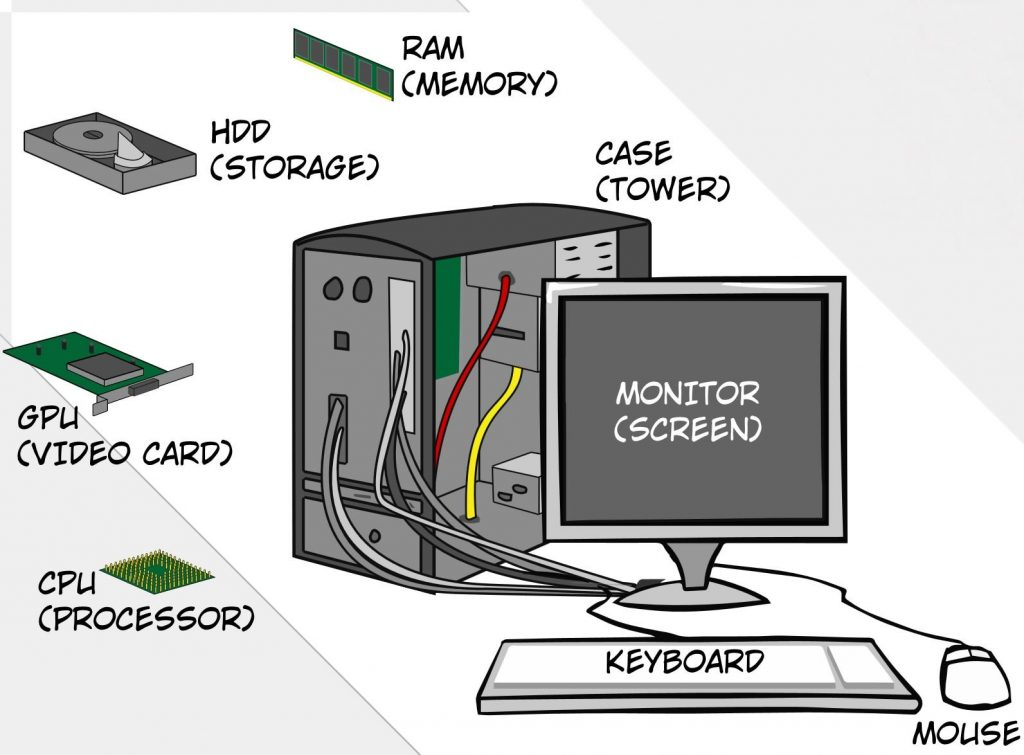
\includegraphics[width=\textwidth]{images/hardware-components.jpg}
	\caption{Examples of hardware components of a personal computer.}
	\label{fig:hardware}
\end{figure}

We will discuss these components in more detail in a later lecture. 

\subsection{Software}

Software (otherwise known as \textit{programs}, \textit{applications}, or \textit{apps}) are organized sets of instructions for controlling the computer.

There are two main classes of software:

\begin{itemize}
	\item Applications: programs allowing the human to interact directly with the computer
	\item Systems software: programs the computer uses to control itself
\end{itemize}

Some familiar applications include:

\begin{itemize}
	\item Microsoft Word: allows the user to edit documents
	\item Mozilla Firefox: connects the user to the World Wide Web
	\item iTunes: organizes and plays music files
\end{itemize}

While applications allow the user to interact with the computer, systems software keeps the computer running. The operating system (OS) is the most common example of systems software, and it schedules tasks and manages storage of data.

We will dive deeper into the details of both applications and systems software in Chapter \ref{ch:hardware_software}.

\subsection{Data}
Data is information of any kind. One key facet of computers is their ability to reliably store massive quantities of data for a long time. Another is the speed with which they can do calculations on data once they receive instructions from a human user.

While humans can understand data with a wide variety of perceptions (taste,
smell, hearing, touch, sight), computers read and write everything internally as
\textit{bits}, sequences of 0s and 1s.

Computers have software and hardware which allow them to convert their internal 0s and 1s into text, numerals, and images displayed on a monitor, as well as sounds which can be played through a speaker.

Similarly, computers have hardware and software that convert information from
the real world into bits: a microphone converts sound, a camera converts pictures, and a text editor converts character symbols.

\subsection{Users}

Of course, there would be no data and no meaningful calculations without the human user. Computers are ultimately tools for making humans more powerful.

As we will see in the next section, different types of computers have different roles for the user.

\section{Types of computers}

\subsection{Supercomputers}

Supercomputers are the most powerful computers out there. They are used for problems that take along time to calculate. They are rare because of their size and expense, and therefore primarily used by big organizations like universities, corporations, and the government.

The user of a supercomputer typically gives the computer a list of instructions, and allows the supercomputer to run on its own over the course of hours or days to complete its task.

Supercomputers generally become ``super'' by combining the capabilities of many different regular computers together. Programming a supercomputer effectively requires an advanced technique called parallel programming, which instructs a group of computers on how to share the work for a task and complete it cooperatively.\endnote{https://insidehpc.com/2018/11/new-top500-list-lead-doe-supercomputers/}

\begin{marginfigure}
	\centering
	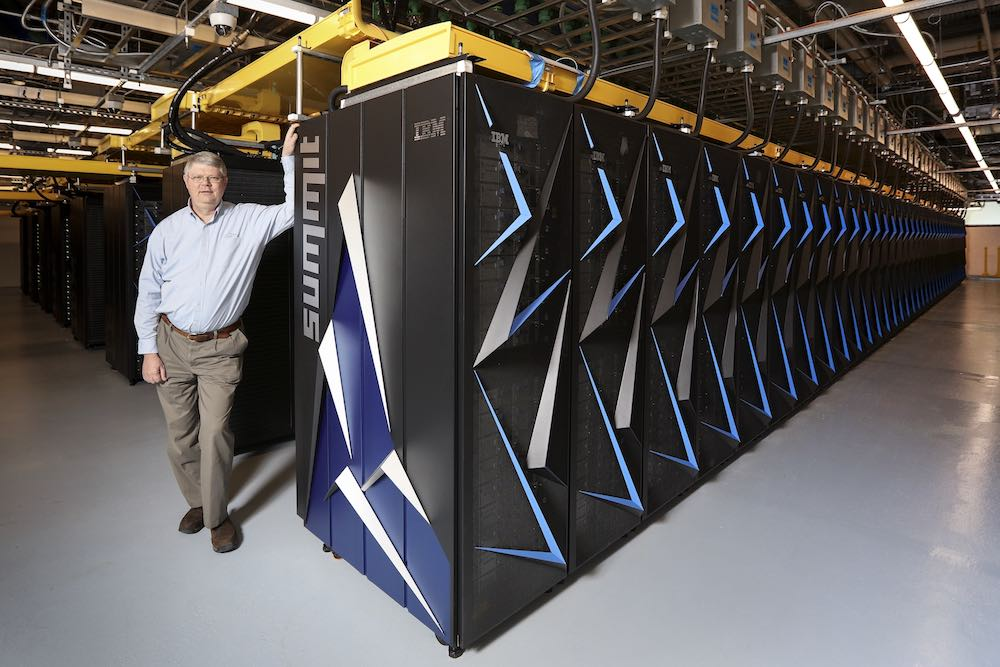
\includegraphics[width=\textwidth]{images/supercomputer.jpg}
	\caption{Summit, a world-class supercomputing cluster at Oak Ridge National Laboratory in Tennessee.}
	\label{fig:supercomputer}
\end{marginfigure}

\subsection{Mainframe computers}
Although not as powerful as supercomputers, mainframe computers can handle more data and run much faster than a typical personal computer. Often, they are given instructions only periodically by computer programmers, and then run on their own for months at a time to store and process incoming data. For example, census number-crunching, consumer statistics, and transactions processing all use mainframe computers.

\subsection{Personal computers}
These are the familiar computers we use to interact with applications every day. Full-size desktop computers and laptop computers are examples.

\subsection{Embedded computers}
In the modern ``digital'' age, nearly all devices we use have computers embedded within them. From cars to washing machines to watches to heating systems, most everyday appliances have a computer within them that allows them to function.

\subsection{Mobile computers}
In the past two decades, mobile computing devices such as smartphones have exploded in popularity, and become nearly as capable as standalone personal computers for many tasks.

\exercisesection

\pgfoonew \maze=new maze()

\begin{marginfigure}[4cm]
  \centering
    \begin{tikzpicture}[scale=.37,flag/.style={scale=.37},turt/.style={scale=.37}]
        \maze.drawMaze();
        \maze.drawTurt();
    \end{tikzpicture}
    \caption{An example maze. The roboturt starts at the box in the bottom left facing toward the top of the page. We need to get it to the box with the finish flags at the top right.}
    \label{fig:graph-paper}
\end{marginfigure}

\begin{exercise}

For this exercise you are going to program a robotic turtle (``roboturt'') to complete a maze. The roboturt accepts two commands:  ``Turn Left [number]'' (TL[n]) and ``Move Forwards [number]'' (MF[n]). The command TL tells the roboturt to change its direction without moving out of its box (and note that 3 lefts can make a right). MF tells the roboturt to step into the box in front of it. For example, the following commands would tell the roboturt to complete the example maze shown in Figure \ref{fig:graph-paper}: MF[4], TL[3], MF[6], TL[1], MF[3], TL[3], MF[3], TL[1], MF[4]. A visual representation of the roboturt following these commands is in Figure \ref{fig:turtle_sequence}.

Get a piece of graph paper, and draw your own maze on it. Make sure to draw a roboturt in the starting box in whatever direction you want it to start in, and a flag at the finish box. You may refer to the maze in Figure \ref{fig:graph-paper} as an example. 
  
First create a list of commands that tells the robot to complete your own maze. Then do the same for another student's maze. Compare your command sequences. 

What types of commands could have made this easier? Could your robot solve
arbitrary mazes? What types of commands would be helpful for making your robot
solve any maze?\safemarginnote[-2cm]{Hint: what happens if the roboturt always follows the wall to its right?}
\end{exercise}


\begin{figure}
  \centering
    \begin{tikzpicture}[scale=0.3,flag/.style={scale=.3},turt/.style={scale=.3}]
        \begin{scope}
            \maze.drawMaze();
            \maze.MF(4);
        \end{scope}
        \begin{scope}[xshift=13cm]
            \maze.drawMaze();
            \maze.TL(3);
        \end{scope}
        \begin{scope}[xshift=26cm]
            \maze.drawMaze();
            \maze.MF(6);
        \end{scope}
        \begin{scope}[yshift=-13cm]
            \maze.drawMaze();
            \maze.TL(1);
        \end{scope}
        \begin{scope}[xshift=13cm,yshift=-13cm]
            \maze.drawMaze();
            \maze.MF(3);
        \end{scope}
        \begin{scope}[xshift=26cm,yshift=-13cm]
            \maze.drawMaze();
            \maze.TL(3);
        \end{scope}
        \begin{scope}[yshift=-26cm]
            \maze.drawMaze();
            \maze.MF(3);
        \end{scope}
        \begin{scope}[xshift=13cm,yshift=-26cm]
            \maze.drawMaze();
            \maze.TL(1);
        \end{scope}
        \begin{scope}[xshift=26cm,yshift=-26cm]
            \maze.drawMaze();
            \maze.MF(4);
        \end{scope}
    \end{tikzpicture}
    %\includegraphics{maze2.png}
   % \includegraphics{maze3.png}
    \caption{A visual representation of what happens when the roboturt follows the commands (MF[4], TL[3], MF[6], TL[1], MF[3], TL[3], MF[3], TL[1], MF[4]).}
    \label{fig:turtle_sequence}
\end{figure}

\begin{exercise}
Imagine a scenario in which you have to describe how to draw a simple house (example shown in Figure~\ref{fig:house-drawing}) to a friend over the phone step-by-step. Is the instruction ``Draw a square with a triangle on top'' sufficient? What instructions would you give to obtain an accurate drawing? 
\end{exercise}

\begin{figure}
  \centering
    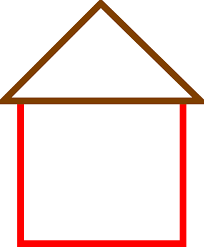
\includegraphics[width=.32\textwidth]{images/simple_house.png}
    \caption{An example of a simple house.}
    \label{fig:house-drawing}
\end{figure}

\begin{exercise}
What are some other tasks a computer can accomplish?
\end{exercise}

\begin{exercise}
  Think about building a simple video game. What are the hardware, software, and
  data needed for this game? What would be the minimal hardware, and what
  hardware would you need to add features like voice chat or online play? What
  types of computers would best run this game? Why?

  Do the same for a text editor and an ATM machine. 
\end{exercise}


\referencessection

\textit{Computer Science: An Interdisciplinary Approach}, Robert Sedgewick and Kevin Wayne.

University of Wisconsin-Madison CS 202 Lectures, Andrea Arpaci-Dusseau.\\http://pages.cs.wisc.edu/~dusseau/Classes/CS202-F11/

\theendnotes
